\chapter{Tabela Comparativa}
\label{tabelacomparativa}

A princípio, o objetivo deste projeto é desenvolver uma aeronave competitiva.
No caso, a competitividade ou qualidade de um projeto aeronáutico pode ser quantificada por meio de duas abordagens.
A primeira tem como objeto de estudo as diversas características apresentadas pela aeronave devido às soluções de engenharia desenvolvidas para atender a necessidade do mercado.
A segunda abordagem avalia a competitividade também em termos de participação no mercado, o que pode ser traduzido como o número de aeronaves em operação e custo operacional.

A proposta desta seção é avaliar, por meio da análise de uma tabela comparativa, as aeronaves que atendem as diretrizes gerais apresentadas na introdução sem adicionar restrições quanto ao sucesso do projeto no mercado da aviação.
Ou seja, utiliza-se da primeira abordagem para analisar as aeronaves que são potenciais competidoras do projeto.
Já a próxima seção tem como objetivo avaliar as aeronaves mais competitivas sob critério de participação no mercado atual.

As aeronaves selecionadas para a construção da tabela comparativa são:
\begin{multicols}{2}
  \begin{enumerate}
    \item Piaggio P180 Avanti
    \item Aerospatiale N 262 Fregate a Mohawk 298
    \item Embraer EMB120 Brasilia
    \item Douglas DC-3
    \item Fairchild Dornier 328JET
    \item Curtis C46 Commando
    \item Short 360
    \item Bombardier Dash 8 Q200
    \item Dornier 328
    \item Convair 240
    \item Let L-610
    \item Douglas DC-4
    \item Casa CN235
    \item Casa/IPTN CN235
    \item Handley Page Herald
    \item Embraer ERJ145
    \item Antonov An-24
    \item ATR 42-600
    \item Bombadier Dash 8 Q300
    \item Bombardier CRJ200
    \item Canadair CL-600 Regional Jet CRJ-100 \& 200
    \item Fokker 50
    \item IPTN N-25050
    \item Hawker Siddeley HS-748
    \item Antonov An-140
    \item Convair 340
    \item Convair 440
    \item Fokker F-27
    \item Douglas DC-6
    \item Convair 580
    \item Saab 2000
    \item Xian MA60
    \item Ilyushin 114
    \item ATR 72-600
    \item Embraer E170
    \item BAe 146-100 / Avro RJ70
    \item Bombadier Dash 8 Q400
  \end{enumerate}
\end{multicols}

Geralmente, uma aeronave comercial tem sua competitividade determinada em termos de desempenho e custo operacional, sendo então plausível a escolha dos seguintes parâmetros para avaliar as soluções de projeto desenvolvidas para atender o mercado de aviação regional:
\begin{multicols}{2}
  \begin{enumerate}
    \item Número de Passageiros - Pax
    \item Tipo do Motor
    \item Número de motores
    \item Modelo do Motor
    \item Potência Total (\si{kW})
    \item Empuxo (\si{kN})
    \item Teto de serviço (\si{ft})
    \item Alcance (\si{nm})
    \item Velocidade Horizontal Máxima (\si{kts})
    \item Velocidade de Cruzeiro (\si{kts})
    \item Envergadura da Asa (\si{m})
    \item Alongamento
    \item Área da asa (\si{m^2})
    \item Comprimento da Aeronave (\si{m})
    \item Altura da Aeronave (\si{m})
    \item MTOW (\si{kg})
    \item Peso Vazio (\si{kg})
    \item Carga Paga (\si{kg})
    \item Distância de decolagem (\si{m})
    \item Preço (milhões USD)
    \item Ano de referência para o preço
    \item Número total de pedidos
    \item Ano de referência para total de pedidos
  \end{enumerate}
\end{multicols}

A tabela comparativa com os dados das aeronaves selecionadas se encontra no Anexo A.
A partir dos dados coletados, decidiu-se construir um gráfico para cada parâmetro listado com o objetivo de identificar qual a tendência apresentada pelas aeronaves do segmento regional, sendo elas agrupadas de acordo com o grupo-motopropulsor.
As figuras \ref{fig:alcance} a \ref{fig:comprimento} apresentam os resultados obtidos, e em seguida tem-se a análise referente a cada parâmetro investigado.
Elas apresentam uma reta de regressão linear para cada tipo de grupo moto-propulsor, assim como uma área sombreada representando um intervalo de confiança de 68\% --- um desvio padrão de uma distribuição gaussiana.

\begin{figure}
\centering
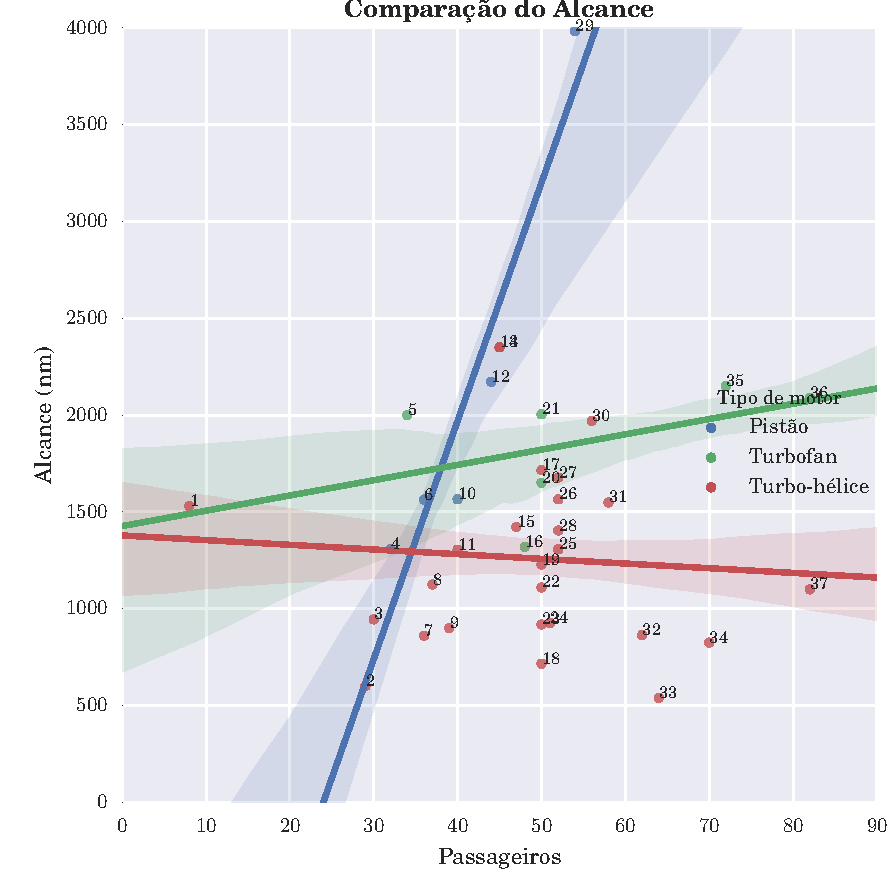
\includegraphics{../autogenerated/graficos_comparativos/alcance.pdf}
\caption[Comparação do alcance]{A média do alcance das aeronaves turbo-hélice e jato é de 1500\si{nmi}.
Os jatos possuem alcance ligeiramente superior aos turbo-hélice, provavelmente devido ao seu melhor desempenho em cruzeiro (maior teto e velocidade), o que torna esse tipo de avião naturalmente mais adequado a voos mais longos.
O aumento acentuado do alcance com o número de passageiros apresentado pelas aeronaves a pistão deve-se ao fato de que mesmo com poucos passageiros elas eram utilizadas para voos longos, já que a tecnologia da época, assim como o uso de propulsão convencional, dificultava a fabricação de aviões de grande porte.}
\label{fig:alcance}
\end{figure}

\begin{figure}
\centering
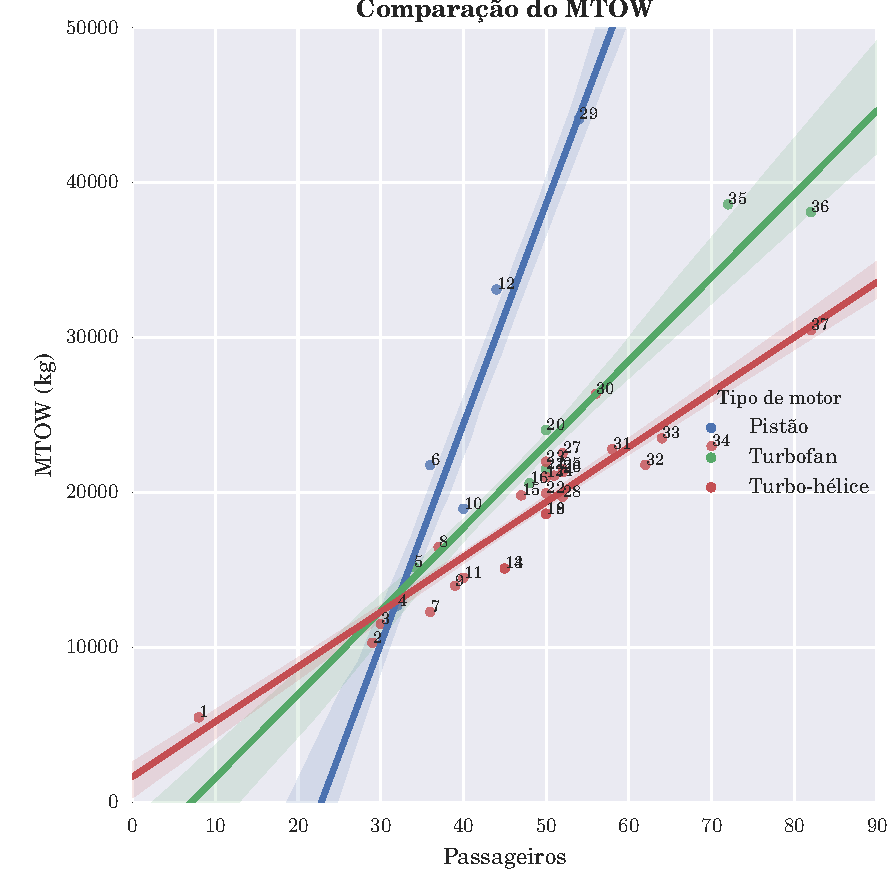
\includegraphics{../autogenerated/graficos_comparativos/mtow.pdf}
\caption[Comparação do MTOW]{O MTOW versus número de passageiros para aeronaves com motor a pistão indica que neste tipo de grupo moto-propulsor a aeronave deve transportar mais peso por passageiro do que os outros motores.
Isso se justifica também pelo fato de que as aeronaves a pistão pesquisadas são antigas e, portanto, têm tecnologias ultrapassadas que implicam em mais peso vazio.
Já uma comparação entre turbo-hélice e turbofan indica que o primeiro grupo moto-propulsor transporta menos peso por passageiro do que o segundo.
Isso fica evidente pela inclinação das curvas, ou seja: quanto menor a inclinação, mais passageiros são transportados por um mesmo MTOW.
Isso implica que as aeronaves turbo-hélices pesquisadas tendem ser mais leves que as aeronaves turbofan para um mesmo número de passageiros.
Uma justificativa seria a questão estrutural, visto que uma aeronave turbofan tem um envelope de voo maior, o que implica em maiores cargas e, logo, em uma estrutura mais pesada.
Além disso, um motor turbofan tende a ser mais pesado que um turbo-hélice.}
\label{fig:mtow}
\end{figure}

% GEOVANA
\begin{figure}
\centering
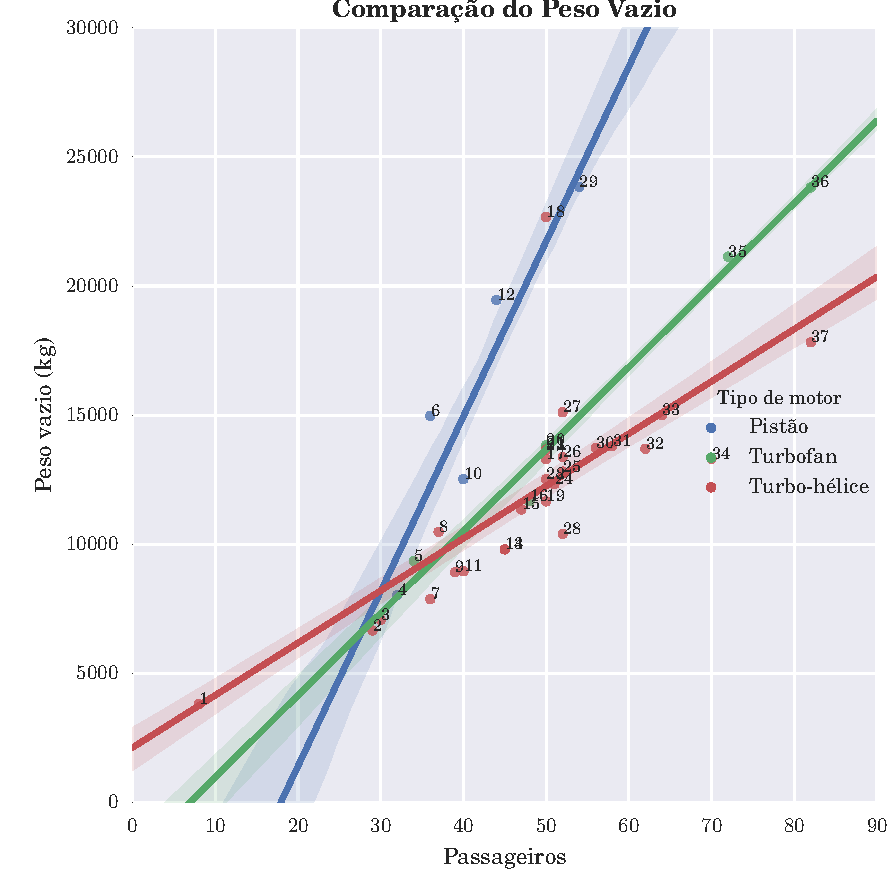
\includegraphics{../autogenerated/graficos_comparativos/pesovazio.pdf}
\caption[Comparação do peso vazio]{O gráfico peso vazio \emph{versus} número de passageiros é consistente com as conclusões do gráfico anterior, visto que as diferenças discutidas em MTOW por número de passageiros entre os grupo moto propulsores se justificam em termos de peso vazio.}
\label{fig:pesovazio}
\end{figure}

\begin{figure}
\centering
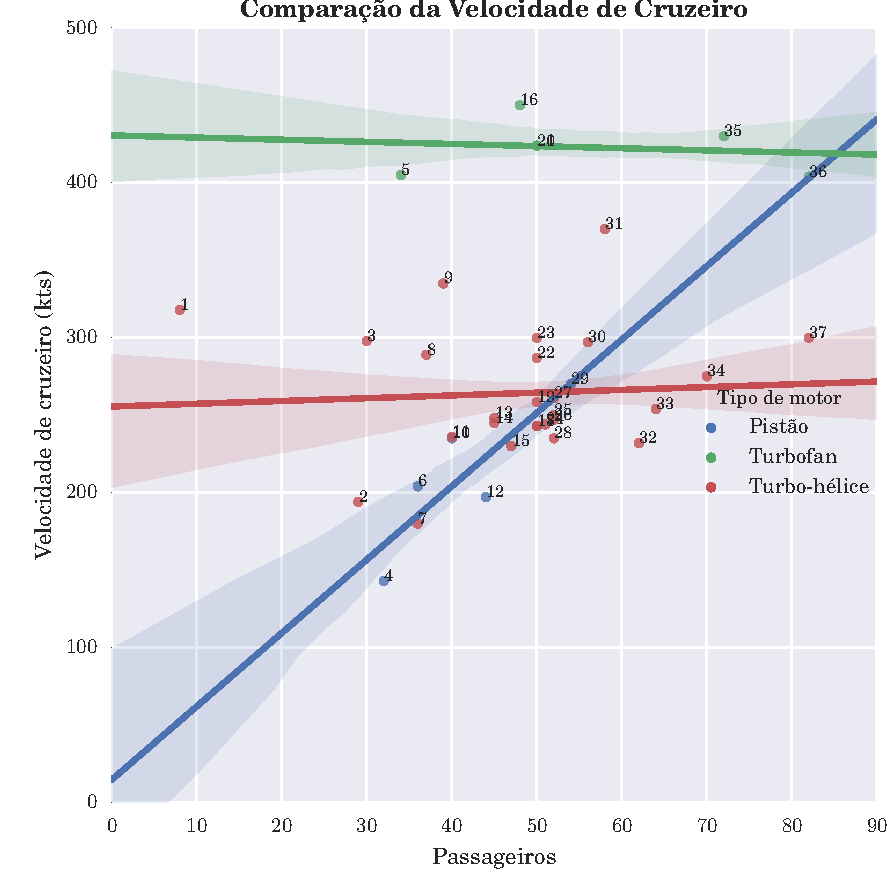
\includegraphics{../autogenerated/graficos_comparativos/vcruzeiro.pdf}
\caption[Comparação da velocidade de cruzeiro]{
A velocidade de cruzeiro dos jatos é substancialmente superior à velocidade de cruzeiro dos turbo-hélices, já que o motor a jato é mais adequado para elevadas altitudes e velocidades.
As aeronaves de tipo turbo-hélice são tão velozes quanto ou mais rápidas que as aeronaves com motor a pistão.
A regressão linear feita para as aeronaves a pistão mostra uma tendência de aumento com o número de passageiros não-compatível com a realidade, ultrapassando inclusive a reta das aeronaves turbo-hélice, devido ao pequeno número de aeronaves desse tipo analisadas.
}
\label{fig:vcruzeiro}
\end{figure}

\begin{figure}
\centering
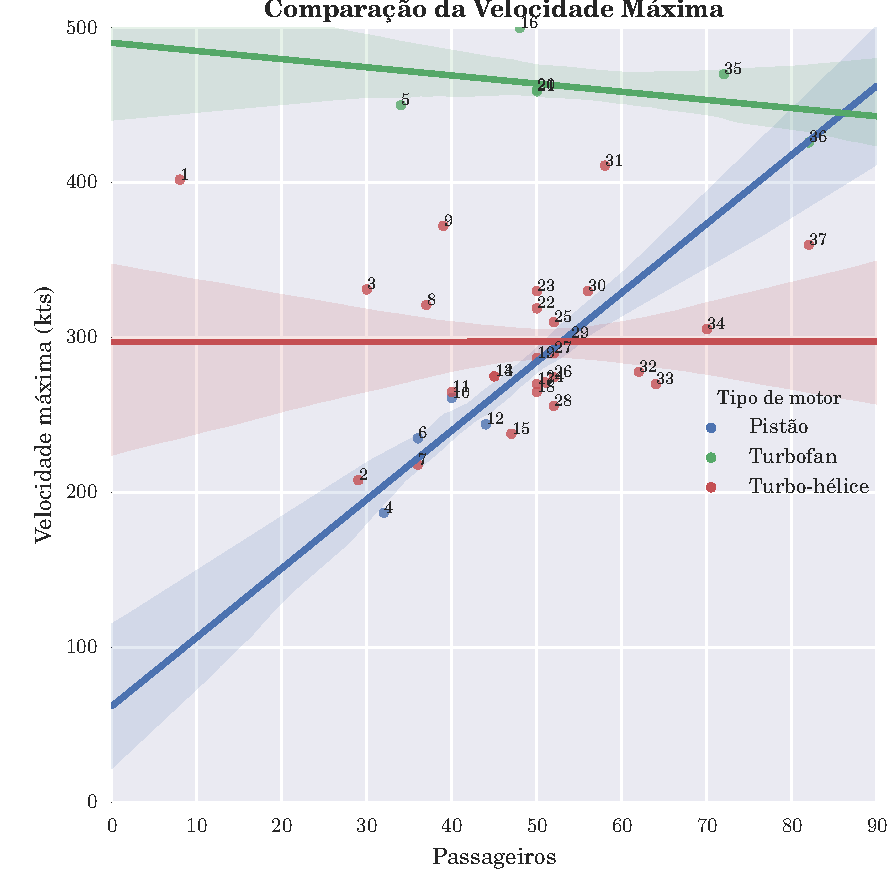
\includegraphics{../autogenerated/graficos_comparativos/vmaxima.pdf}
\caption[Comparação da velocidade máxima]{As tendências observadas aqui são as mesmas da velocidade de cruzeiro (\autoref{fig:vcruzeiro}).}
\label{fig:vmaxima}
\end{figure}

\begin{figure}
\centering
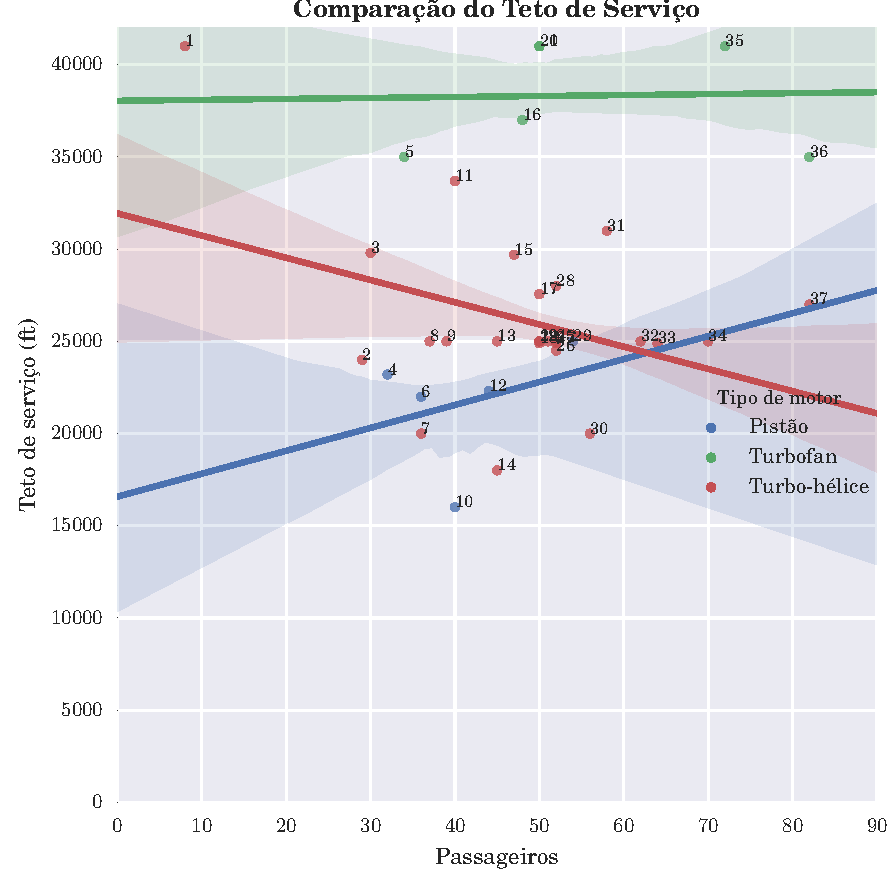
\includegraphics{../autogenerated/graficos_comparativos/teto.pdf}
\caption[Comparação do teto operacional]{
O teto operacional dos jatos é maior que o dos turbo-hélices, que por sua vez é maior do que o das aeronaves com propulsão convencional.
Isso se deve às características inerentes de cada tipo de moto propulsor: jatos operam de forma muito eficiente em altitudes elevadas, e motores a pistão são bastante sensíveis à diminuição da densidade atmosférica.
A propulsão turbo-hélice está em um ponto intermediário. As linhas de regressão não são muito representativas nesse caso, pois há grande variância entre os pontos.
}
\label{fig:teto}
\end{figure}

\begin{figure}
\centering
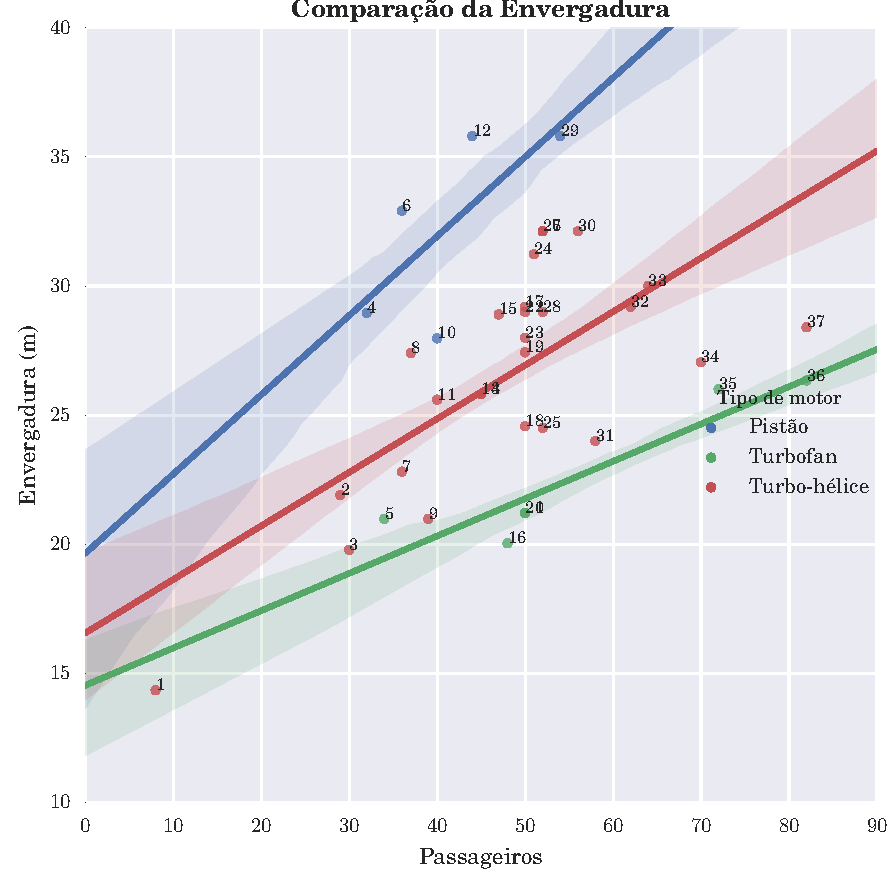
\includegraphics{../autogenerated/graficos_comparativos/envergadura.pdf}
\caption[Comparação da envergadura]{
A envergadura varia com o inverso da velocidade das aeronaves: os jatos voam mais rápido, e por isso precisam de menos área alar, mas também apresentam cargas mais elevadas sobre as asas, o que sugere asas de menor alongamento. Estes dois efeitos contribuem para a redução da envergadura. Os turbo-hélices e as aeronaves a pistão voam mais lentamente, então precisam de maior área alar e desenvolvem menores cargas sobre as asas, permitindo um maior alongamento que, por sua vez, aumenta a eficiência aerodinâmica.
}
\label{fig:envergadura}
\end{figure}

\begin{figure}
\centering
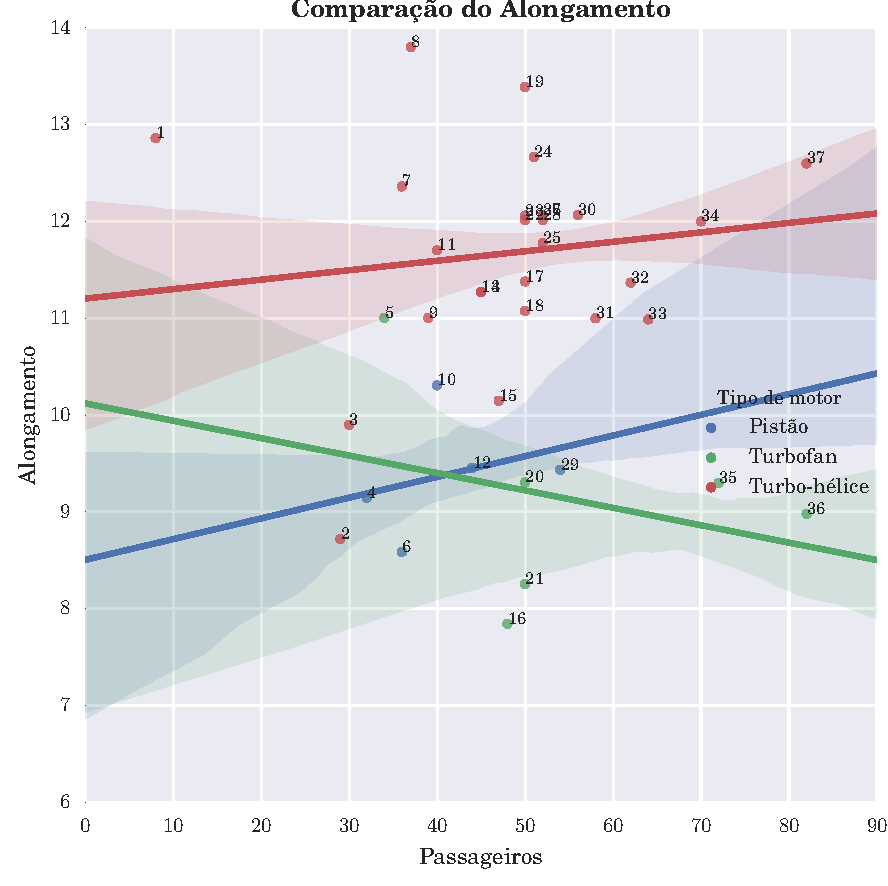
\includegraphics{../autogenerated/graficos_comparativos/alongamento.pdf}
\caption[Comparação do alcance]{
Como discutido na \autoref{fig:envergadura}, o afilamento é determinado pelas cargas e resistência das estruturas da asa, pois do ponto de vista aerodinâmico, quanto mais alongada, melhor a asa. As maiores cargas enfrentadas pelos jatos, devido à maior velocidade, fazem com que suas asas sejam menos alongadas do que as dos turbo-hélice. O alongamento das aeronaves a pistão é comparável ao das turbo-hélices: apesar de voarem mais lentamente, as aeronaves a pistão são mais antigas, e por isso os materiais usados em sua fabricação são menos resistentes.
}
\label{fig:alongamento}
\end{figure}

\begin{figure}
\centering
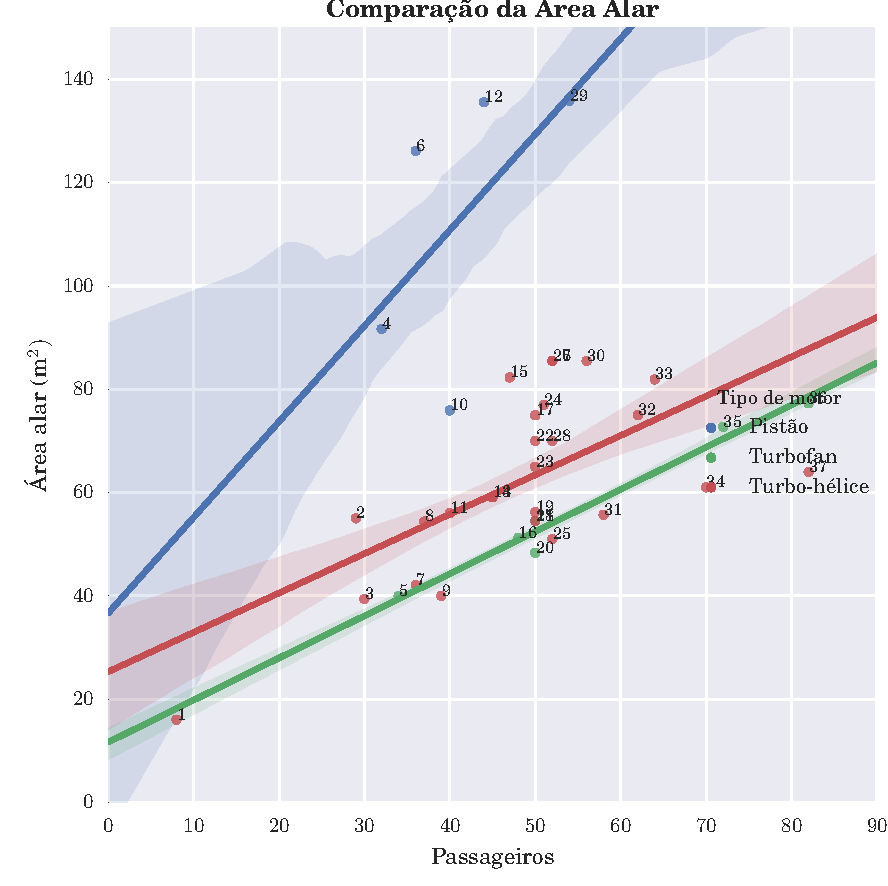
\includegraphics{../autogenerated/graficos_comparativos/area.pdf}
\caption[Comparação da área]{Assim como a envergadura (\autoref{fig:envergadura}), a área alar aumenta com a diminuição na velocidade de operação. Entretanto, aqui a alteração não é tão evidente entre jatos e turbo-hélice, já que o maior alongamento dos turbo-hélice aumenta sua eficiência aerodinâmica, o que compensa, em parte, as velocidades mais baixas. As aeronaves a pistão possuem área alar notavelmente mais elevada devido novamente a serem mais antigas. Os avanços tecnológicos permitiram um aumento da eficiência aerodinâmica das asas, o que diminuiu a área alar necessária.}
\label{fig:area}
\end{figure}

%Geovana
\begin{figure}
\centering
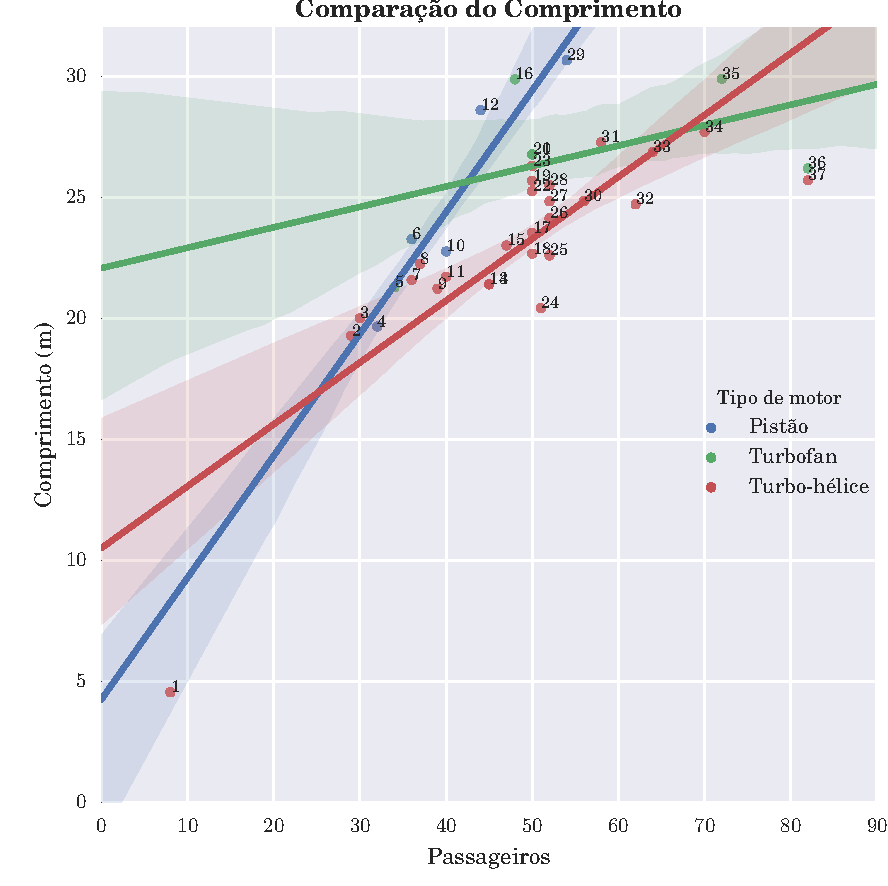
\includegraphics{../autogenerated/graficos_comparativos/comprimento.pdf}
\caption[Comparação da altura]{Em relação à altura das aeronaves, pode-se notar que os aviões com turbofan e turbo-hélice apresentam uma tendência similar na altura \emph{versus} o número de passageiros.
Porém, as aeronaves com grupo moto-propulsor turbo-hélice geralmente são asa alta e têm empenagens na configuração em T, o que pode justificar o fato de estes aviões serem mais altos.
Em relação ao motor a pistão, constata-se que as aeronaves apresentam um aumento mais acentuado na altura com o aumento do número de passageiros.
Uma das justificativas é em relação a empenagem vertical, visto que nas aeronaves com tecnologias antigas, as superfícies sustentadores tendem a ser maiores para um mesmo número de passageiros, já que o peso vazio é maior. Além disso, todas as aeronaves com motor a pistão analisadas são asa baixa e, portanto, o trem de pouso deve ser alto o suficiente de forma que as hélices não atinjam o chão.}
\label{fig:comprimento}
\end{figure}


% Geovana
\begin{figure}
\centering
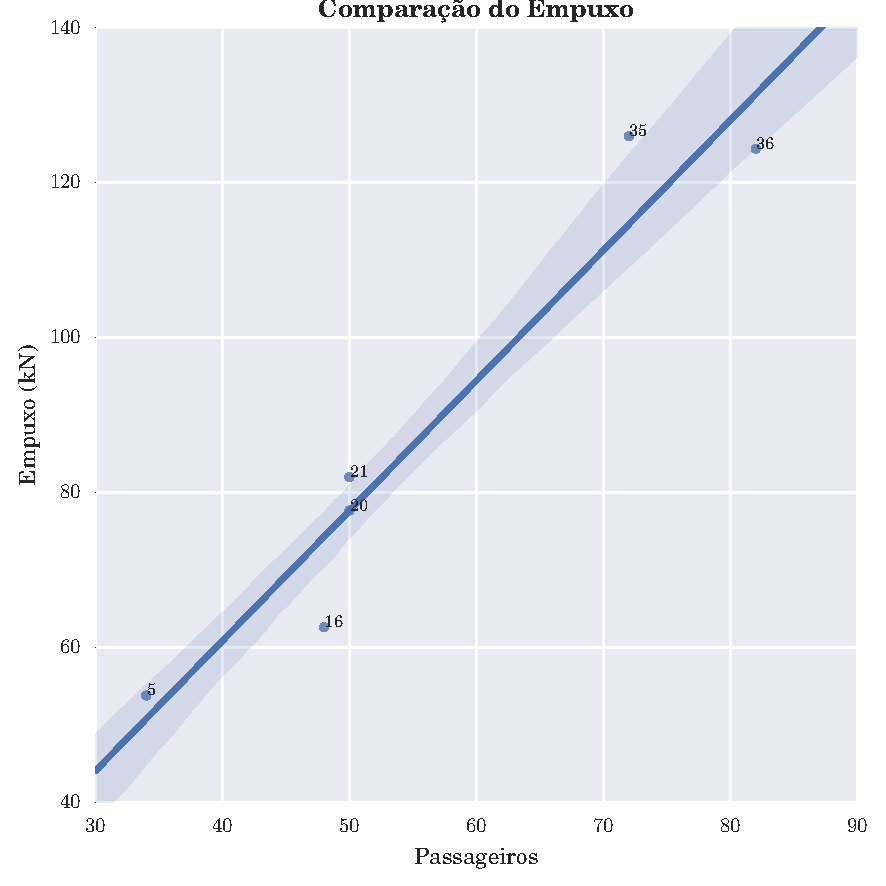
\includegraphics{../autogenerated/graficos_comparativos/empuxo.pdf}
\caption[Comparação do empuxo para aeronaves com turbofan]{O empuxo versus número de passageiros para aeronaves turbofan seguem uma relação aproximadamente linear. Ou seja, a regressão linear representa consideravelmente a relação entre estes dois parâmetros.}
\label{fig:empuxo}
\end{figure}

% Laura
\begin{figure}
\centering
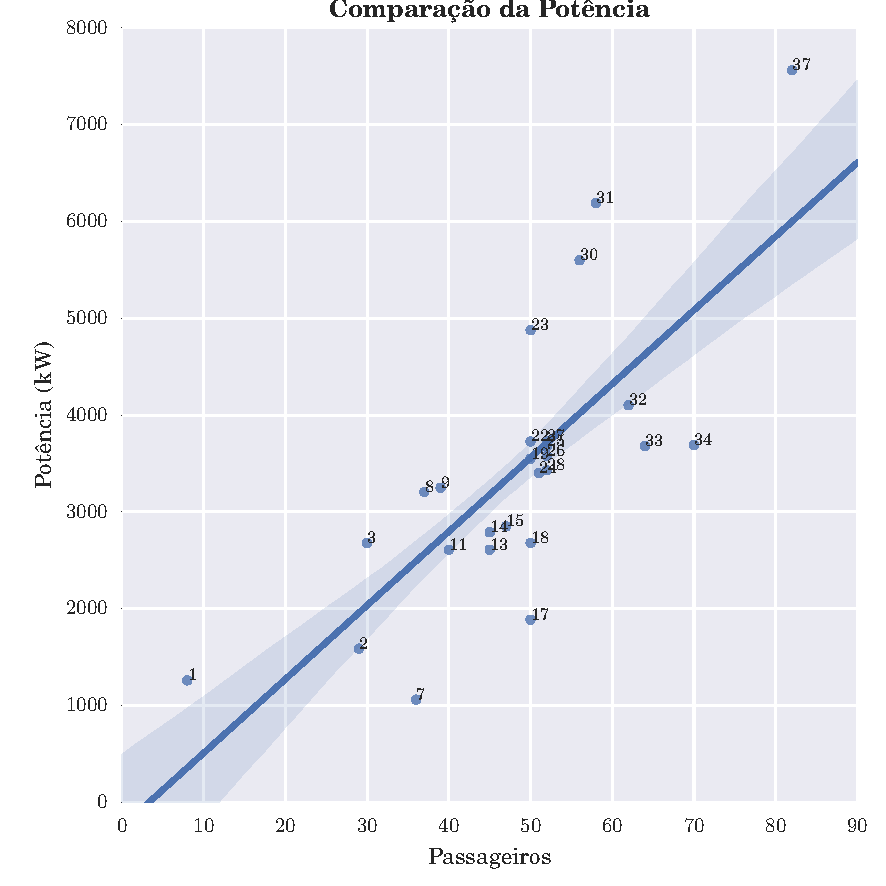
\includegraphics{../autogenerated/graficos_comparativos/potencia.pdf}
\caption[Comparação da potência para aeronaves com turbo-hélice]{Já no caso das aeronaves turbo-hélices, a regressão linear não representa muito bem a relação entre a potência e o número de passageiros. Isso se deve ao fato de que devido a grande diferença entre os anos de fabricação das aeronaves, a tecnologia dos motores varia bastante o que indica uma oportunidade no estudo de novas tecnologias para este tipo de motor.}
\label{fig:potencia}
\end{figure}

\begin{sidewaystable}[p]
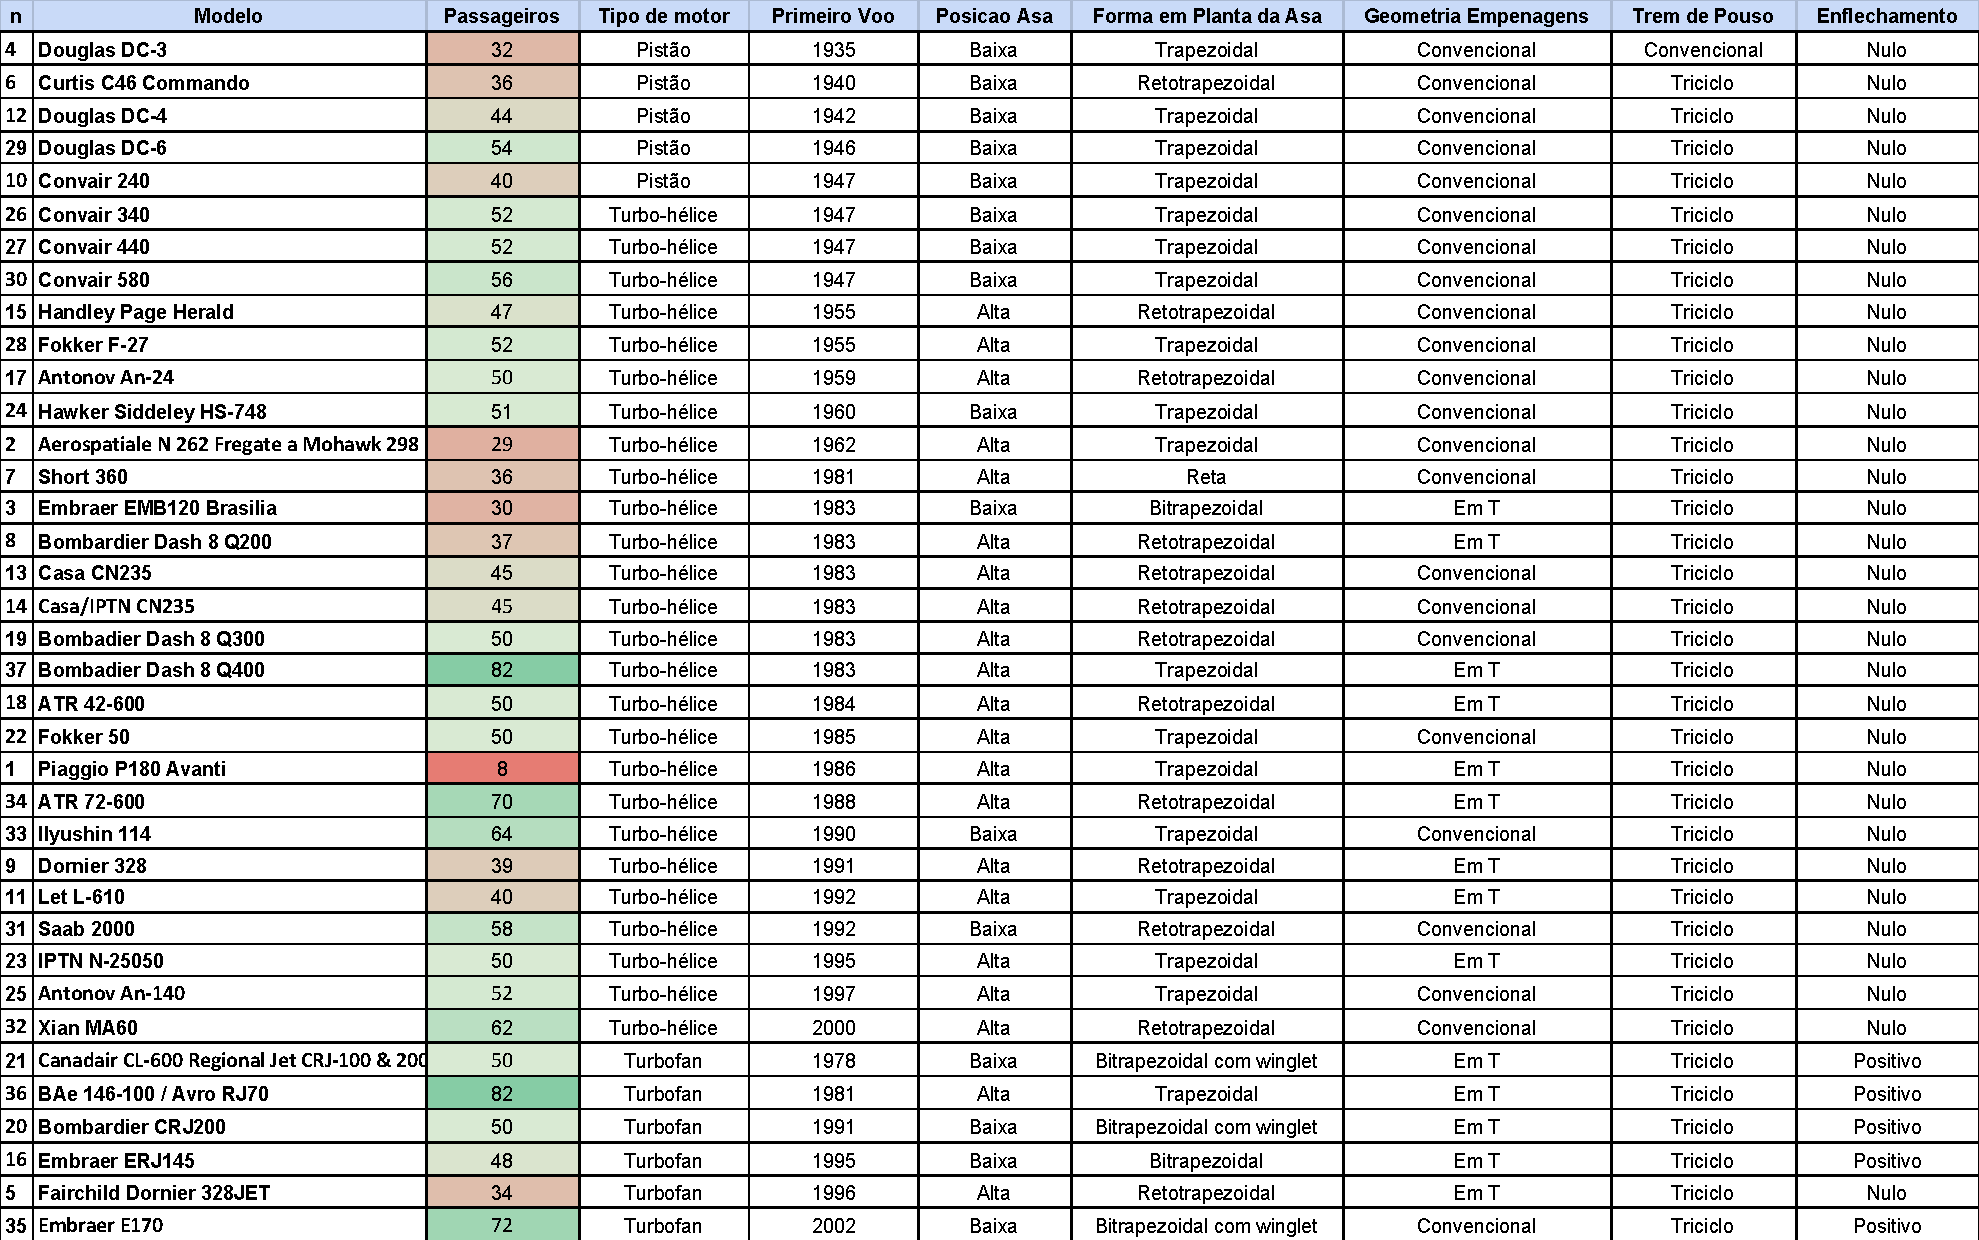
\includegraphics[width=24cm]{Tabela_Comparativa_CONCEITOS.pdf}
\caption{Soluções conceituais das aeronaves em análise}
\label{conceitos_tabela}
\end{sidewaystable}

\clearpage
As informações em relação as soluções conceituais como posição da asa, geometria das empenagens, geometria do trem de pouso, enflechamento e forma em planta da asa estão na \autoref{conceitos_tabela}. Além disso, também tem-se a informação do ano do primeiro voo de cada aeronave e qual o respectivo grupo moto-propulsor.

Como pode ser observado da tabela, todos aviões com propulsão convencional são antigos e datam da década de 40. Isso justifica a diferença considerável encontrada para peso vazio dessas aeronaves em comparação com as aeronaves mais recentes turbofan e turbo-hélice. Além disso, o único avião com trem de pouso convencional dos 37 analisados é o Douglas DC-3, datado de 1935, o que evidencia a dominância do trem de pouso triciclo no projeto de aeronaves.

Outra fato interessante é que todos os aviões turbofan, exceto o E170 (maior avião turbofan analisado com capacidade para 70 passageiros), tem seu conjunto de empenagens em T. Neste caso, o motor geralmente é posicionado na parte traseira da fuselagem e este posicionamento não exige por norma que um reforço na fuselagem seja feito em caso de despalhetamento do motor, ou seja, esta configuração permite um menor peso vazio para aeronaves em torno de 50 passageiros.

No caso de aeronaves turbo-hélice com motor na asa, há a predominância de asa alta, o que se justifica pelo fato de que a hélice do motor não pode tocar o chão. Este problema é resolvido tanto com o posicionamento da asa, tanto com o tamanho do trem de pouso. Além disso, como os aviões turbo-hélice voam em um regime de Mach subsônico, não há a necessidade de enflechamento para reduzir arrasto devido às ondas de choque e a forma em planta da asa é predominantemente bitrapezoidal. Esta configuração garante bom desempenho aerodinâmico além de um baixo custo de fabricação em comparação com as de geometrias mais complexas de asa.

Com a \autoref{conceitos_tabela}, pode-se principalmente avaliar as diferenças conceituais entre aeronave turbofan e turbo-hélice. Portanto, conclui-se que predominantemente aeronaves turbofan apresentam enflechamento, asa baixa, empenagens em T e motores na fuselagem. Já as aeronaves turbo-hélice, em geral, apresentam asa alta, enflechamento nulo, empenagens tanto em T quanto convencionais e motores na asa.
